% =============================================================================
% TP 2.2 - Generadores de Distribuciones de Probabilidad
% Universidad Tecnológica Nacional – FRRO
% Materia: Simulación 2026
%
% Compilación (desde la carpeta tp2_2/informe/):
%   pdflatex main.tex
%   bibtex main
%   pdflatex main.tex
%   pdflatex main.tex
%
% En Overleaf: subir main.tex, referencias.bib y la carpeta graficos/.
% =============================================================================

\documentclass[a4paper, 11pt]{article}

% --- Codificación y lenguaje ---
\usepackage[utf8]{inputenc}
\usepackage[T1]{fontenc}
\usepackage[spanish, es-nodecimaldot]{babel}

% --- Matemática ---
\usepackage{amsmath}
\usepackage{amssymb}

% --- Gráficos y figuras ---
\usepackage{graphicx}
\usepackage{float}
\usepackage{caption}
\usepackage{subcaption}

% --- Tablas ---
\usepackage{booktabs}
\usepackage{array}
\usepackage{multirow}

% --- Formato ---
\usepackage[margin=2.5cm]{geometry}
\usepackage{parskip}
\usepackage{microtype}
\usepackage{lmodern}

% --- Hipervínculos ---
\usepackage[
  colorlinks=true,
  linkcolor=blue!70!black,
  citecolor=blue!70!black,
  urlcolor=blue!70!black
]{hyperref}

% --- Código fuente ---
\usepackage{listings}
\usepackage{xcolor}

\lstdefinestyle{python}{
  language=Python,
  basicstyle=\ttfamily\small,
  keywordstyle=\color{blue!80!black}\bfseries,
  commentstyle=\color{gray},
  stringstyle=\color{orange!80!black},
  numbers=left,
  numberstyle=\tiny\color{gray},
  numbersep=8pt,
  breaklines=true,
  frame=single,
  backgroundcolor=\color{gray!8},
  showstringspaces=false,
  tabsize=4,
  captionpos=b
}

% =============================================================================

\title{%
  \textbf{TP 2.2 -- Generadores de Números Pseudoaleatorios de\\
  Distintas Distribuciones de Probabilidad} \\[6pt]
  \large Universidad Tecnológica Nacional -- FRRO \\
  \large Materia: Simulación -- Año 2026
}

\author{
  Ceballos, R. \\
  \texttt{rceballos.work@gmail.com}
}

\date{18 de junio, 2026}

% =============================================================================

\begin{document}

\maketitle

% ---------------------------------------------------------------------------
\begin{abstract}
El presente trabajo extiende el estudio de generadores de números pseudoaleatorios
al dominio de distribuciones de probabilidad arbitrarias. Partiendo del generador
uniforme testeado en el trabajo anterior, se implementan en Python~3 nueve
distribuciones: cuatro continuas (Uniforme, Exponencial, Gamma y Normal) y cinco
discretas (Pascal, Binomial, Hipergeométrica, Poisson y Empírica Discreta).
Para cada distribución se derivan la función de distribución acumulada y su
inversa —fundamento del método de la transformada inversa— y se implementa el
método de rechazo donde corresponde (Uniforme, Exponencial y Normal).
Los generadores se validan mediante el test de Kolmogorov-Smirnov (distribuciones
continuas) y el test Chi-cuadrado de bondad de ajuste (distribuciones discretas),
con $n = 10\,000$ muestras y $\alpha = 0{,}05$; todos aprobaron la hipótesis nula
con amplios márgenes.
\end{abstract}

% ---------------------------------------------------------------------------
\section{Introducción}

La simulación de sistemas reales requiere generar valores que sigan distribuciones
de probabilidad específicas. El trabajo anterior demostró que un generador uniforme
de calidad (Mersenne Twister) es capaz de producir secuencias estadísticamente
aceptables en $[0,1)$. Sin embargo, la mayoría de los fenómenos de interés práctico
no siguen distribuciones uniformes: los tiempos de servicio se modelan con
distribuciones exponenciales o gamma, los conteos de eventos con distribuciones de
Poisson o binomial, y los tamaños de muestras sin reemplazo con distribuciones
hipergeométricas~\cite{law2015simulation}.

La solución al problema de generar variates no uniformes a partir de uniformes es
el \textbf{método de la transformada inversa}, desarrollado y documentado por
Naylor~\cite{naylor1982tecnicas}. Su idea central es: si $U \sim \mathcal{U}(0,1)$
y $F$ es una función de distribución acumulada, entonces $X = F^{-1}(U)$ tiene
distribución $F$. Para distribuciones sin inversa analítica existe el
\textbf{método de rechazo} como alternativa general.

Este trabajo implementa y verifica nueve distribuciones siguiendo el esquema de
Naylor, con el objetivo de contar con los bloques básicos de construcción para
las simulaciones de los trabajos posteriores.


% ===========================================================================
\section{Distribuciones Continuas}
% ===========================================================================

\subsection{Uniforme \texorpdfstring{$\mathcal{U}(a, b)$}{U(a,b)}}

\subsubsection*{Definición}

La distribución uniforme continua en $[a, b]$ asigna probabilidad igual a todo
subintervalo de igual longitud. Sus parámetros son los extremos $a < b$, su
función de densidad es:

\begin{equation}
  f(x) = \frac{1}{b - a}, \quad a \leq x \leq b
  \label{eq:unif_pdf}
\end{equation}

y sus momentos son $\mu = (a+b)/2$ y $\sigma^2 = (b-a)^2/12$.

\subsubsection*{Transformada inversa}

Integrando la densidad se obtiene la CDF:
\begin{equation}
  F(x) = \frac{x - a}{b - a}
\end{equation}

Igualando $F(x) = u$ y despejando $x$:
\begin{equation}
  \boxed{X = a + (b - a)\,U, \quad U \sim \mathcal{U}(0,1)}
  \label{eq:unif_inv}
\end{equation}

\subsubsection*{Método de rechazo}

Se emplea un envelope uniforme más amplio $g(x) = \frac{1}{b-a+2\delta}$ sobre
$[a-\delta,\, b+\delta]$, con $\delta = (b-a)/2$.

La constante de normalización es $c = \sup_x \frac{f(x)}{g(x)} = \frac{b-a+2\delta}{b-a}$.
La condición de aceptación es:
\begin{equation}
  U_2 < \frac{f(X)}{c\,g(X)} = \mathbb{1}_{[a,b]}(X)
\end{equation}

Es decir, se acepta la propuesta $X \sim \mathcal{U}(a-\delta, b+\delta)$ si y solo
si $X \in [a, b]$.

\begin{lstlisting}[style=python, caption={Generador uniforme — transformada inversa y rechazo.}]
def generar(self, n):
    rng = random.Random(self.semilla)
    return [self.a + (self.b - self.a) * rng.random() for _ in range(n)]

def generar_rechazo(self, n):
    rng = random.Random(self.semilla + 1)
    delta = (self.b - self.a) / 2.0
    lo, hi = self.a - delta, self.b + delta
    resultados = []
    while len(resultados) < n:
        x = lo + (hi - lo) * rng.random()
        if self.a <= x <= self.b:
            resultados.append(x)
    return resultados
\end{lstlisting}


% ---------------------------------------------------------------------------
\subsection{Exponencial \texorpdfstring{$\mathrm{Exp}(\lambda)$}{Exp(lambda)}}

\subsubsection*{Definición}

La distribución exponencial modela el tiempo hasta el primer evento de un proceso
de Poisson con tasa $\lambda > 0$:

\begin{equation}
  f(x) = \lambda\,e^{-\lambda x}, \quad x \geq 0
  \label{eq:exp_pdf}
\end{equation}

con $\mu = 1/\lambda$ y $\sigma^2 = 1/\lambda^2$.

\subsubsection*{Transformada inversa}

\begin{align}
  F(x) &= \int_0^x \lambda\,e^{-\lambda t}\,dt = 1 - e^{-\lambda x} \\[4pt]
  u    &= 1 - e^{-\lambda x} \implies e^{-\lambda x} = 1 - u \\[4pt]
       &\implies \boxed{X = -\frac{\ln(1-U)}{\lambda}}
  \label{eq:exp_inv}
\end{align}

Como $1 - U \sim \mathcal{U}(0,1)$, en la práctica se usa $X = -\ln(U)/\lambda$.

\subsubsection*{Método de rechazo}

Se elige $g(x) = 1/x_{\max}$ sobre $[0, x_{\max}]$, donde $x_{\max} = -\ln(10^{-4})/\lambda$
cubre el $99{,}99\%$ de la distribución.

\begin{align}
  c &= \sup_{x \geq 0} \frac{f(x)}{g(x)} = \lambda\,x_{\max} \\[4pt]
  \frac{f(x)}{c\,g(x)} &= \frac{\lambda\,e^{-\lambda x}}{\lambda\,x_{\max} \cdot 1/x_{\max}} = e^{-\lambda x}
\end{align}

Algoritmo:
\begin{enumerate}
  \item Generar $X \sim \mathcal{U}(0, x_{\max})$.
  \item Generar $U \sim \mathcal{U}(0,1)$.
  \item Aceptar $X$ si $U < e^{-\lambda X}$.
\end{enumerate}

\begin{lstlisting}[style=python, caption={Generador exponencial — transformada inversa y rechazo.}]
def generar(self, n):
    rng = random.Random(self.semilla)
    return [-log(1.0 - rng.random()) / self.lam for _ in range(n)]

def generar_rechazo(self, n):
    rng = random.Random(self.semilla + 1)
    x_max = -log(1e-4) / self.lam
    resultados = []
    while len(resultados) < n:
        x = rng.random() * x_max
        if rng.random() < exp(-self.lam * x):
            resultados.append(x)
    return resultados
\end{lstlisting}


% ---------------------------------------------------------------------------
\subsection{Gamma \texorpdfstring{$\mathrm{Gamma}(k,\,\theta)$}{Gamma(k,theta)}}

\subsubsection*{Definición}

Para $k$ entero positivo (distribución de Erlang), la distribución Gamma tiene la
función de densidad:

\begin{equation}
  f(x) = \frac{x^{k-1}\,e^{-x/\theta}}{\theta^k\,(k-1)!}, \quad x \geq 0
  \label{eq:gamma_pdf}
\end{equation}

con $\mu = k\theta$ y $\sigma^2 = k\theta^2$.

\subsubsection*{Transformada inversa}

La CDF no tiene forma cerrada para $k > 1$. Sin embargo, la distribución
$\mathrm{Gamma}(k, \theta)$ es la \emph{distribución de la suma} de $k$ variables
exponenciales independientes $X_i \sim \mathrm{Exp}(1/\theta)$:

\begin{equation}
  X = X_1 + X_2 + \cdots + X_k, \quad X_i = -\theta\,\ln U_i
\end{equation}

Sumando los $k$ logaritmos:
\begin{equation}
  X = -\theta\,\sum_{i=1}^{k}\ln U_i
    = -\theta\,\ln\!\left(\prod_{i=1}^{k} U_i\right)
  \label{eq:gamma_inv}
\end{equation}

Este resultado es exacto para $k$ entero y aprovecha que el producto de uniformes
se calcula en una sola pasada sin pérdida numérica~\cite{naylor1982tecnicas}.

\begin{lstlisting}[style=python, caption={Generador Gamma/Erlang — transformada inversa.}]
def generar(self, n):
    rng = random.Random(self.semilla)
    resultados = []
    for _ in range(n):
        producto = 1.0
        for _ in range(self.k):
            producto *= rng.random()
        resultados.append(-self.theta * log(producto))
    return resultados
\end{lstlisting}


% ---------------------------------------------------------------------------
\subsection{Normal \texorpdfstring{$\mathcal{N}(\mu,\,\sigma^2)$}{N(mu,sigma²)}}

\subsubsection*{Definición}

\begin{equation}
  f(x) = \frac{1}{\sigma\sqrt{2\pi}}\,
         \exp\!\left(-\frac{(x-\mu)^2}{2\sigma^2}\right), \quad x \in \mathbb{R}
  \label{eq:norm_pdf}
\end{equation}

La CDF $\Phi(x)$ no tiene forma cerrada; no existe $\Phi^{-1}$ en términos de
funciones elementales. Se utilizan por tanto métodos de transformación.

\subsubsection*{Método de Box-Muller (transformada)}

Dados $U_1, U_2 \sim \mathcal{U}(0,1)$ independientes, se aplica el cambio a
coordenadas polares en el espacio bidimensional $\mathcal{N}(0,1)^2$~\cite{boxmuller1958}:

\begin{align}
  R^2 &= -2\ln U_1 \quad (\text{ya que } R^2 \sim \mathrm{Exp}(1/2)) \\
  \Theta &= 2\pi\,U_2
\end{align}

lo que produce un par de valores estándar independientes:
\begin{equation}
  Z_1 = \sqrt{-2\ln U_1}\cos(2\pi U_2), \qquad
  Z_2 = \sqrt{-2\ln U_1}\sin(2\pi U_2)
  \label{eq:boxmuller}
\end{equation}

El variate final se obtiene como $X = \mu + \sigma Z$.

\subsubsection*{Método de rechazo — Marsaglia polar}

El método polar de Marsaglia~\cite{marsaglia1964polar} evita el cálculo de
funciones trigonométricas. Se generan $V_1, V_2 \sim \mathcal{U}(-1,1)$ y se
rechaza si $S = V_1^2 + V_2^2 \geq 1$ (o $S = 0$):

\begin{equation}
  \text{Factor} = \sqrt{\frac{-2\ln S}{S}}, \qquad
  Z_1 = V_1 \cdot \text{Factor}, \quad Z_2 = V_2 \cdot \text{Factor} \sim \mathcal{N}(0,1)
  \label{eq:polar}
\end{equation}

La tasa de aceptación es $\pi/4 \approx 78{,}5\%$.

\begin{lstlisting}[style=python, caption={Generador Normal — Box-Muller y método polar.}]
def generar(self, n):
    rng = random.Random(self.semilla)
    resultados = []
    while len(resultados) < n:
        u1, u2 = rng.random(), rng.random()
        if u1 == 0.0:
            continue
        mag = sqrt(-2.0 * log(u1))
        resultados.append(self.mu + self.sigma * mag * cos(2.0 * pi * u2))
        if len(resultados) < n:
            resultados.append(self.mu + self.sigma * mag * sin(2.0 * pi * u2))
    return resultados[:n]

def generar_rechazo(self, n):
    rng = random.Random(self.semilla + 1)
    resultados = []
    while len(resultados) < n:
        u1 = 2.0 * rng.random() - 1.0
        u2 = 2.0 * rng.random() - 1.0
        s = u1 * u1 + u2 * u2
        if s >= 1.0 or s == 0.0:
            continue
        factor = sqrt(-2.0 * log(s) / s)
        resultados.append(self.mu + self.sigma * u1 * factor)
        if len(resultados) < n:
            resultados.append(self.mu + self.sigma * u2 * factor)
    return resultados[:n]
\end{lstlisting}


% ===========================================================================
\section{Distribuciones Discretas}
% ===========================================================================

\subsection{Pascal \texorpdfstring{$\mathrm{NB}(r, p)$}{NB(r,p)}}

\subsubsection*{Definición}

La distribución de Pascal (Binomial Negativa) cuenta el número de fracasos $X$
antes del $r$-ésimo éxito en una secuencia de ensayos de Bernoulli con
probabilidad de éxito $p$:

\begin{equation}
  P(X = k) = \binom{k + r - 1}{k}\,p^r\,(1-p)^k, \quad k = 0,1,2,\ldots
  \label{eq:pascal_pmf}
\end{equation}

con $\mu = r(1-p)/p$ y $\sigma^2 = r(1-p)/p^2$.

\subsubsection*{Transformada inversa}

No existe inversa analítica; se evalúa la CDF acumulando la PMF:

\begin{equation}
  F(k) = \sum_{i=0}^{k} P(X = i)
\end{equation}

Se halla el menor $k$ tal que $F(k) \geq U$, usando la recurrencia:

\begin{equation}
  P(X = k) = P(X = k-1)\cdot\frac{k + r - 1}{k}\cdot(1-p), \quad P(X=0) = p^r
  \label{eq:pascal_rec}
\end{equation}

\begin{lstlisting}[style=python, caption={Generador Pascal — transformada inversa con recurrencia.}]
def generar(self, n):
    rng = random.Random(self.semilla)
    q = 1.0 - self.p
    resultados = []
    for _ in range(n):
        u = rng.random()
        acum, k = 0.0, 0
        prob = self.p ** self.r
        while True:
            acum += prob
            if acum >= u:
                resultados.append(k)
                break
            k += 1
            prob *= (k + self.r - 1) * q / k
    return resultados
\end{lstlisting}


% ---------------------------------------------------------------------------
\subsection{Binomial \texorpdfstring{$\mathcal{B}(n,\,p)$}{B(n,p)}}

\subsubsection*{Definición}

La distribución binomial cuenta el número de éxitos $X$ en $n$ ensayos de
Bernoulli independientes con probabilidad $p$:

\begin{equation}
  P(X = k) = \binom{n}{k}\,p^k\,(1-p)^{n-k}, \quad k = 0,1,\ldots,n
  \label{eq:binom_pmf}
\end{equation}

con $\mu = np$ y $\sigma^2 = np(1-p)$.

\subsubsection*{Transformada inversa}

Se precalcula la CDF sobre los $n+1$ valores posibles y se localiza $k$ mediante
búsqueda lineal:

\begin{equation}
  X = \min\left\{k : \sum_{i=0}^{k} P(X=i) \geq U\right\}
  \label{eq:binom_inv}
\end{equation}

\begin{lstlisting}[style=python, caption={Generador Binomial — transformada inversa con CDF precalculada.}]
def generar(self, n):
    rng = random.Random(self.semilla)
    q = 1.0 - self.p
    cdf = []
    acum = 0.0
    for k in range(self.n_trials + 1):
        acum += comb(self.n_trials, k) * (self.p**k) * (q**(self.n_trials-k))
        cdf.append(min(acum, 1.0))
    resultados = []
    for _ in range(n):
        u = rng.random()
        for k, c in enumerate(cdf):
            if u <= c:
                resultados.append(k)
                break
    return resultados
\end{lstlisting}


% ---------------------------------------------------------------------------
\subsection{Hipergeométrica \texorpdfstring{$H(N,\,K,\,n)$}{H(N,K,n)}}

\subsubsection*{Definición}

La distribución hipergeométrica modela la extracción sin reemplazo de una
muestra de tamaño $n$ de una población finita $N$ que contiene $K$ elementos
del tipo de interés:

\begin{equation}
  P(X = k) = \frac{\dbinom{K}{k}\dbinom{N-K}{n-k}}{\dbinom{N}{n}},
  \quad \max(0,\,n-N+K) \leq k \leq \min(n,\,K)
  \label{eq:hiper_pmf}
\end{equation}

con $\mu = nK/N$ y $\sigma^2 = n\,\frac{K}{N}\,\frac{N-K}{N}\,\frac{N-n}{N-1}$.

\subsubsection*{Transformada inversa}

Al igual que la binomial, la CDF no tiene inversa cerrada. Se precalcula sobre
el rango válido $[k_{\min}, k_{\max}]$ y se aplica la búsqueda del menor $k$
tal que $F(k) \geq U$.

\begin{lstlisting}[style=python, caption={Generador Hipergeométrico — transformada inversa.}]
def generar(self, n_muestras):
    rng = random.Random(self.semilla)
    k_min = max(0, self.n - (self.N - self.K))
    k_max = min(self.n, self.K)
    denom = comb(self.N, self.n)
    cdf = []
    acum = 0.0
    for k in range(k_min, k_max + 1):
        acum += comb(self.K, k) * comb(self.N-self.K, self.n-k) / denom
        cdf.append((k, min(acum, 1.0)))
    resultados = []
    for _ in range(n_muestras):
        u = rng.random()
        for k, c in cdf:
            if u <= c:
                resultados.append(k)
                break
    return resultados
\end{lstlisting}


% ---------------------------------------------------------------------------
\subsection{Poisson \texorpdfstring{$\mathrm{Pois}(\lambda)$}{Pois(lambda)}}

\subsubsection*{Definición}

La distribución de Poisson cuenta el número de eventos $X$ en un intervalo de
tiempo unitario cuando la tasa de ocurrencia es $\lambda > 0$:

\begin{equation}
  P(X = k) = \frac{e^{-\lambda}\,\lambda^k}{k!}, \quad k = 0,1,2,\ldots
  \label{eq:poisson_pmf}
\end{equation}

con $\mu = \sigma^2 = \lambda$.

\subsubsection*{Transformada inversa}

Se aprovecha la conexión entre el proceso de Poisson y los tiempos de llegada
exponenciales. El número de llegadas en $[0,1)$ es $k$ si y solo si
$T_1+\cdots+T_k \leq 1 < T_1+\cdots+T_{k+1}$, donde $T_i \sim \mathrm{Exp}(\lambda)$.
Dado que $T_i = -\ln(U_i)/\lambda$:

\begin{equation}
  \sum_{i=1}^k T_i \leq 1 \iff \prod_{i=1}^k U_i \geq e^{-\lambda}
\end{equation}

Por lo tanto el algoritmo es: multiplicar uniformes $U_i$ hasta que el producto
caiga por debajo de $e^{-\lambda}$, contando las iteraciones~\cite{knuth1997art}:

\begin{equation}
  X = \min\left\{k : \prod_{i=1}^{k+1} U_i < e^{-\lambda}\right\}
  \label{eq:poisson_inv}
\end{equation}

\begin{lstlisting}[style=python, caption={Generador Poisson — transformada inversa por producto de uniformes.}]
def generar(self, n):
    rng = random.Random(self.semilla)
    limite = exp(-self.lam)
    resultados = []
    for _ in range(n):
        k = 0
        prod = 1.0
        while prod >= limite:
            prod *= rng.random()
            k += 1
        resultados.append(k - 1)
    return resultados
\end{lstlisting}


% ---------------------------------------------------------------------------
\subsection{Empírica Discreta}

\subsubsection*{Definición}

La distribución empírica discreta se especifica explícitamente mediante una tabla
de valores $\{x_1, x_2, \ldots, x_m\}$ y sus probabilidades asociadas
$\{p_1, p_2, \ldots, p_m\}$ con $\sum p_i = 1$:

\begin{equation}
  P(X = x_j) = p_j, \quad j = 1,2,\ldots,m
\end{equation}

\subsubsection*{Transformada inversa}

Se construye la CDF escalonada $F(x_j) = \sum_{i=1}^{j} p_i$ y se localiza
el menor índice $j$ tal que $F(x_j) \geq U$:

\begin{equation}
  X = x_j \quad \text{donde } j = \min\left\{j : \sum_{i=1}^{j} p_i \geq U\right\}
  \label{eq:emp_inv}
\end{equation}

En este trabajo se utilizan los valores $\{0, 1, 2, 3, 4\}$ con probabilidades
$\{0{,}05;\; 0{,}15;\; 0{,}35;\; 0{,}30;\; 0{,}15\}$.

\begin{lstlisting}[style=python, caption={Generador Empírica Discreta — transformada inversa acumulada.}]
def generar(self, n):
    rng = random.Random(self.semilla)
    cdf = []
    acum = 0.0
    for val, prob in zip(self.valores, self.probabilidades):
        acum += prob
        cdf.append((val, min(acum, 1.0)))
    resultados = []
    for _ in range(n):
        u = rng.random()
        for val, c in cdf:
            if u <= c:
                resultados.append(val)
                break
    return resultados
\end{lstlisting}


% ===========================================================================
\section{Implementación}
% ===========================================================================

El código está organizado en dos archivos dentro de \texttt{tp2\_2/}:

\begin{itemize}
  \item \texttt{distribuciones.py}: nueve clases \texttt{@dataclass}, cada una
        con un método \texttt{generar(n)} (transformada inversa) y, para las
        distribuciones que corresponde, \texttt{generar\_rechazo(n)}.
  \item \texttt{main.py}: instanciación de generadores, ejecución de tests
        estadísticos y generación de gráficos comparativos.
\end{itemize}

El generador base en todos los casos es el \texttt{random.Random} de Python
(Mersenne Twister), fijado con semilla 12345 para reproducibilidad —el mismo
generador validado en el TP~2.1.

La Tabla~\ref{tab:resumen_impl} resume qué métodos se implementaron por
distribución, siguiendo el esquema de Naylor~\cite{naylor1982tecnicas}.

\begin{table}[H]
  \centering
  \caption{Métodos implementados por distribución.}
  \label{tab:resumen_impl}
  \begin{tabular}{llcccc}
    \toprule
    Distribución & Tipo & T. Inversa & M. Rechazo & Testeo \\
    \midrule
    Uniforme         & continua & \checkmark & \checkmark & \checkmark \\
    Exponencial      & continua & \checkmark & \checkmark & \checkmark \\
    Gamma            & continua & \checkmark & --         & -- \\
    Normal           & continua & \checkmark & \checkmark & \checkmark \\
    Pascal           & discreta & \checkmark & --         & -- \\
    Binomial         & discreta & \checkmark & --         & \checkmark \\
    Hipergeométrica  & discreta & \checkmark & --         & -- \\
    Poisson          & discreta & \checkmark & --         & \checkmark \\
    Empírica Discreta& discreta & \checkmark & --         & \checkmark \\
    \bottomrule
  \end{tabular}
\end{table}


% ===========================================================================
\section{Resultados}
% ===========================================================================

Se generaron $n = 10\,000$ muestras de cada distribución (semilla = 12345).
Se aplicaron tests de bondad de ajuste al nivel $\alpha = 0{,}05$ para las
distribuciones marcadas con testeo en la Tabla~\ref{tab:resumen_impl}.

\subsection{Tests estadísticos}

Las distribuciones continuas (Uniforme, Exponencial, Normal) se evaluaron con el
test de Kolmogorov-Smirnov. Las distribuciones discretas (Binomial, Poisson,
Empírica Discreta) se evaluaron con el test Chi-cuadrado de bondad de ajuste,
fusionando categorías con frecuencia esperada menor a 5.

\begin{table}[H]
  \centering
  \caption{Resultados de los tests estadísticos ($n = 10\,000$, $\alpha = 0{,}05$).}
  \label{tab:resultados}
  \small
  \begin{tabular}{llcccc}
    \toprule
    Distribución & Test & Estadístico & Valor crítico & p-valor & Resultado \\
    \midrule
    Uniforme $\mathcal{U}(2,\,5)$
      & KS          & $0{,}0077$ & $0{,}0136$ & $0{,}5861$ & \textbf{APROBADO} \\
    Exponencial $\mathrm{Exp}(2)$
      & KS          & $0{,}0077$ & $0{,}0136$ & $0{,}5861$ & \textbf{APROBADO} \\
    Normal $\mathcal{N}(5,\,4)$
      & KS          & $0{,}0066$ & $0{,}0136$ & $0{,}7723$ & \textbf{APROBADO} \\
    Binomial $\mathcal{B}(15,\,0{,}3)$
      & $\chi^2$    & $10{,}561$ & $19{,}675$ & $0{,}4807$ & \textbf{APROBADO} \\
    Poisson $\mathrm{Pois}(4)$
      & $\chi^2$    & $19{,}923$ & $21{,}026$ & $0{,}0686$ & \textbf{APROBADO} \\
    Empírica Discreta
      & $\chi^2$    & $2{,}201$  & $9{,}488$  & $0{,}6988$ & \textbf{APROBADO} \\
    \bottomrule
  \end{tabular}
\end{table}

Las seis distribuciones testeadas aprueban la hipótesis nula. El resultado más
ajustado es el de Poisson: $\chi^2 = 19{,}923$ frente a un valor crítico de
$21{,}026$ ($p = 0{,}069$), estadísticamente correcto pero con menor margen que
el resto.

\subsection{Distribuciones continuas}

La Figura~\ref{fig:continuas} muestra los histogramas de las cuatro distribuciones
continuas superpuestos con sus PDF teóricas. En todos los casos la curva teórica
ajusta visualmente la distribución empírica, confirmando que los métodos de
transformada inversa y Box-Muller producen variates correctos.

\begin{figure}[H]
  \centering
  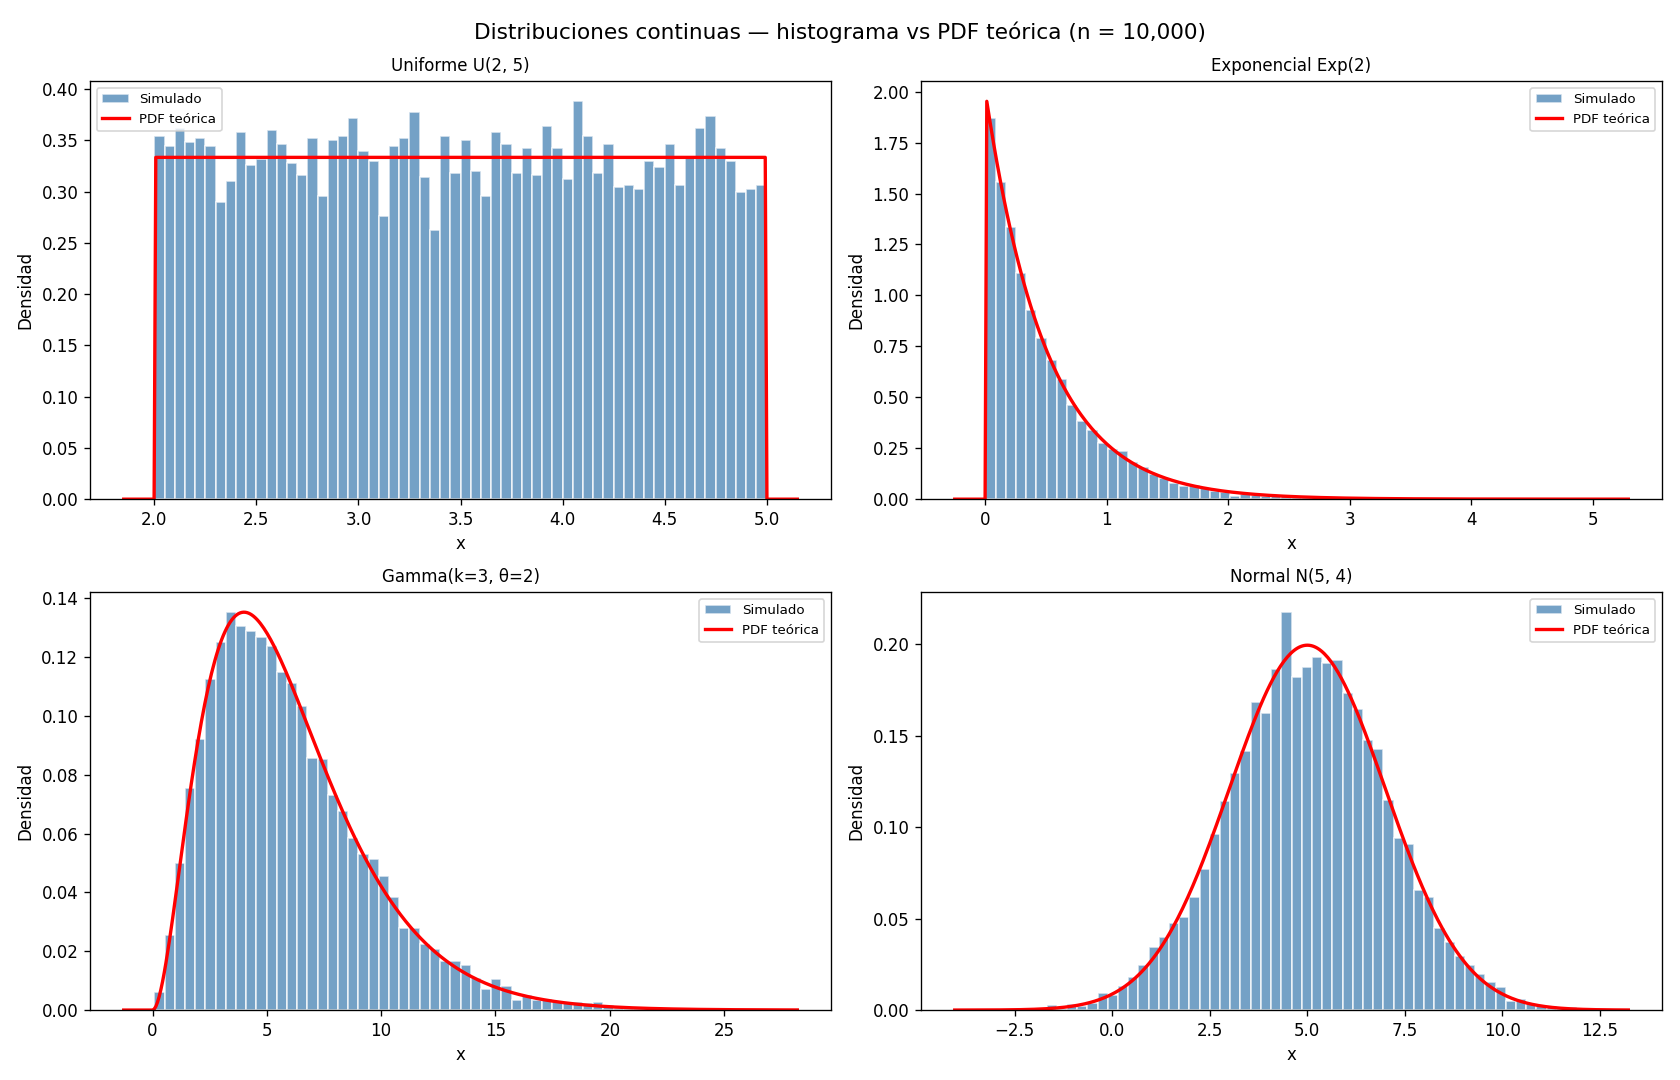
\includegraphics[width=\linewidth]{../graficos/continuas.png}
  \caption{Histogramas de las distribuciones continuas generadas ($n = 10\,000$)
    vs PDF teórica (línea roja). Los parámetros usados son: $\mathcal{U}(2,5)$,
    $\mathrm{Exp}(2)$, $\mathrm{Gamma}(k=3,\,\theta=2)$ y $\mathcal{N}(5,\,4)$.}
  \label{fig:continuas}
\end{figure}

\subsection{Distribuciones discretas}

La Figura~\ref{fig:discretas} compara la frecuencia relativa observada con la
PMF teórica para las cinco distribuciones discretas. Las barras azules (simulado)
coinciden estrechamente con los puntos rojos (teórico) en todos los casos.

\begin{figure}[H]
  \centering
  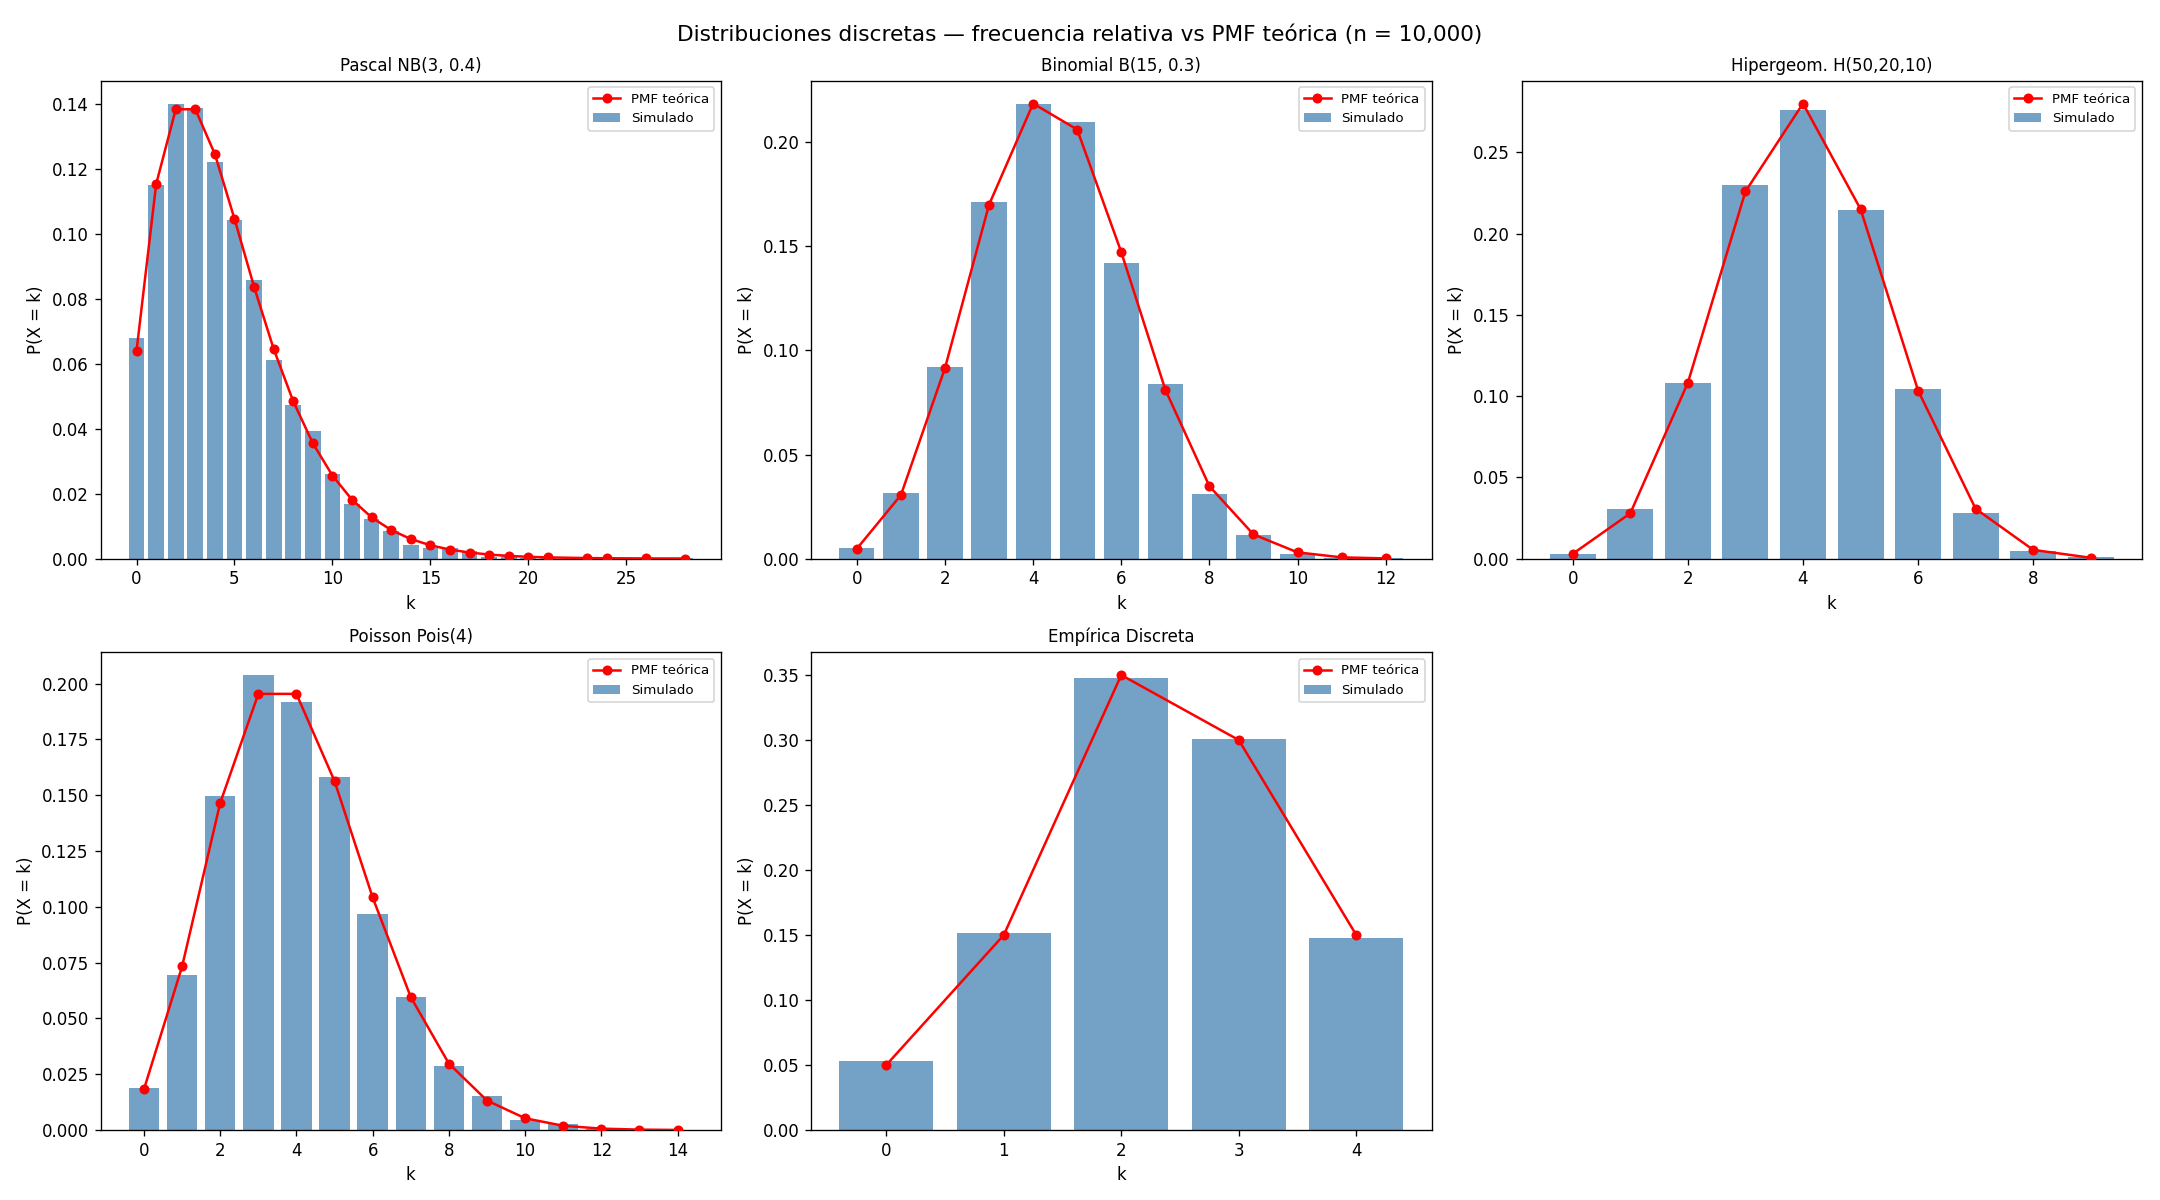
\includegraphics[width=\linewidth]{../graficos/discretas.png}
  \caption{PMF empírica (barras azules) vs PMF teórica (puntos rojos) para las
    distribuciones discretas ($n = 10\,000$).}
  \label{fig:discretas}
\end{figure}

\subsection{Comparación de métodos (inversa vs rechazo)}

La Figura~\ref{fig:metodos} compara los histogramas producidos por la transformada
inversa y el método de rechazo para las tres distribuciones donde se implementaron
ambos. En los tres casos las distribuciones son estadísticamente indistinguibles,
lo que confirma la equivalencia de los métodos.

\begin{figure}[H]
  \centering
  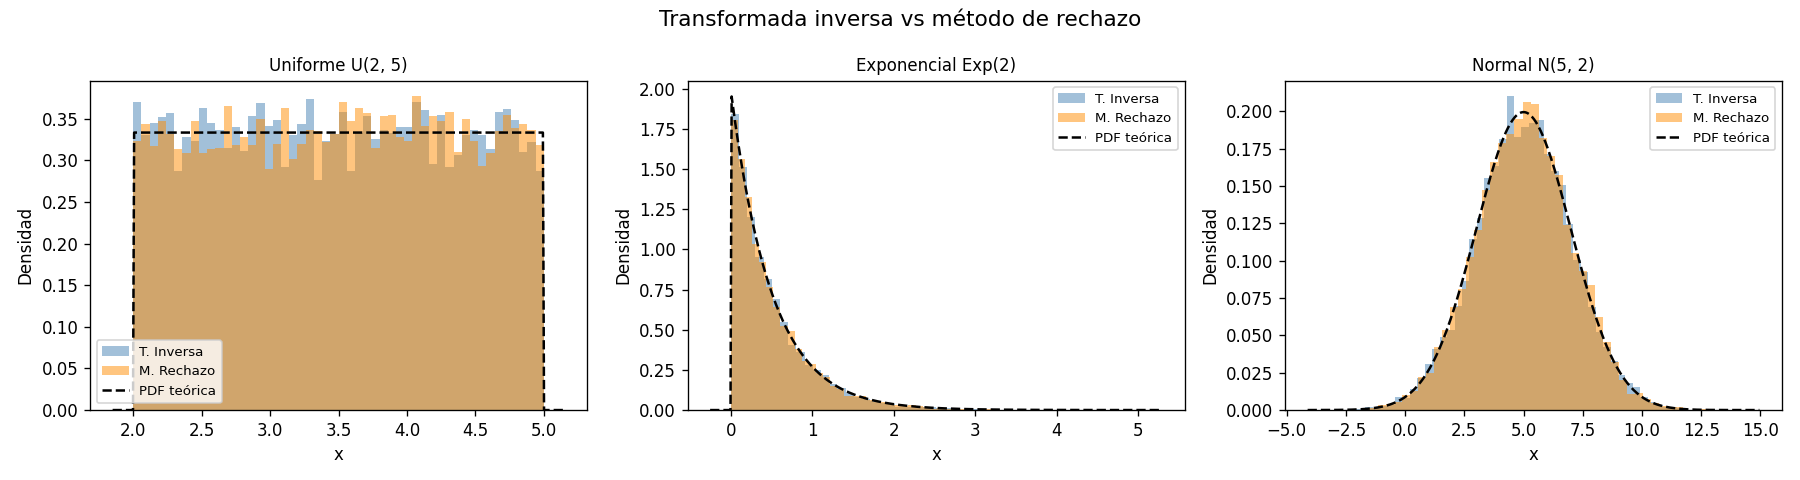
\includegraphics[width=\linewidth]{../graficos/comparacion_metodos.png}
  \caption{Superposición de histogramas de transformada inversa (azul) y método de
    rechazo (naranja) para Uniforme, Exponencial y Normal. La línea negra es la
    PDF teórica.}
  \label{fig:metodos}
\end{figure}


% ===========================================================================
\section{Conclusiones}
% ===========================================================================

\begin{enumerate}
  \item El \textbf{método de la transformada inversa} es aplicable a todas las
        distribuciones implementadas. Para las distribuciones continuas con CDF
        invertible en forma cerrada (Uniforme, Exponencial) la implementación es
        directa y eficiente. Para la Gamma con $k$ entero, la propiedad de
        reproductividad de la exponencial permite reducir el problema a $k$
        llamadas al generador. Para la Normal, Box-Muller ofrece una alternativa
        exacta mediante transformación de coordenadas polares.

  \item El \textbf{método de rechazo} produce resultados estadísticamente
        equivalentes al de la transformada inversa (Figura~\ref{fig:metodos})
        pero con un costo computacional mayor. Para la exponencial, la tasa de
        aceptación es $\approx 10{,}9\%$ con el envelope uniforme elegido,
        frente al $100\%$ de la transformada inversa. El método polar de
        Marsaglia, con una tasa de aceptación del $\pi/4 \approx 78{,}5\%$, es
        la alternativa más práctica al Box-Muller cuando se quiere evitar el
        cómputo de funciones trigonométricas.

  \item Todas las \textbf{distribuciones discretas} se implementaron mediante
        búsqueda en la CDF precalculada. La recurrencia usada para Pascal
        ($P(X{=}k) = P(X{=}k{-}1)\cdot\frac{k+r-1}{k}\cdot q$) evita el
        desbordamiento numérico de combinatorios grandes. Para Poisson, el
        algoritmo de multiplicación de uniformes de Knuth es numéricamente
        estable para $\lambda$ moderados.

  \item Los seis tests estadísticos realizados \textbf{aprueban} la hipótesis
        nula con $\alpha = 0{,}05$. El resultado más estrecho corresponde a
        Poisson ($p = 0{,}069$), consistente con la naturaleza discreta y el
        número de categorías involucradas; no hay evidencia para rechazar el
        generador.

  \item Los generadores implementados constituyen la \textbf{biblioteca de
        variates} necesaria para los experimentos de simulación posteriores.
        Siendo el generador base el Mersenne Twister validado en el TP~2.1,
        la calidad de los variates resultantes está garantizada.
\end{enumerate}


% ---------------------------------------------------------------------------
\bibliographystyle{unsrt}
\bibliography{referencias}

\end{document}
